\chapter{Escenarios}
    \label{chap:six}
    
\section{Ciudad 1. Cruce simple}
\begin{figure}[H]
    \centering
    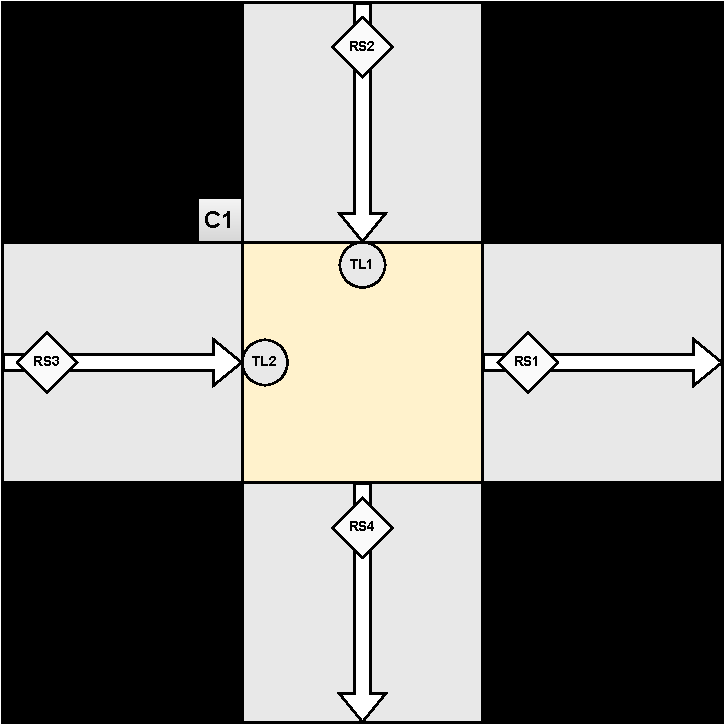
\includegraphics[width=1\linewidth]{text/image/DCruc-CSimple-Topologia.pdf}
    \caption{Topología del cruce simple}
    \label{fig:cruce_simple_topologia}
\end{figure}

\newpage
\section{Ciudad 2. Matriz de cruces simples 2x1}
\begin{figure}[H]
    \centering
    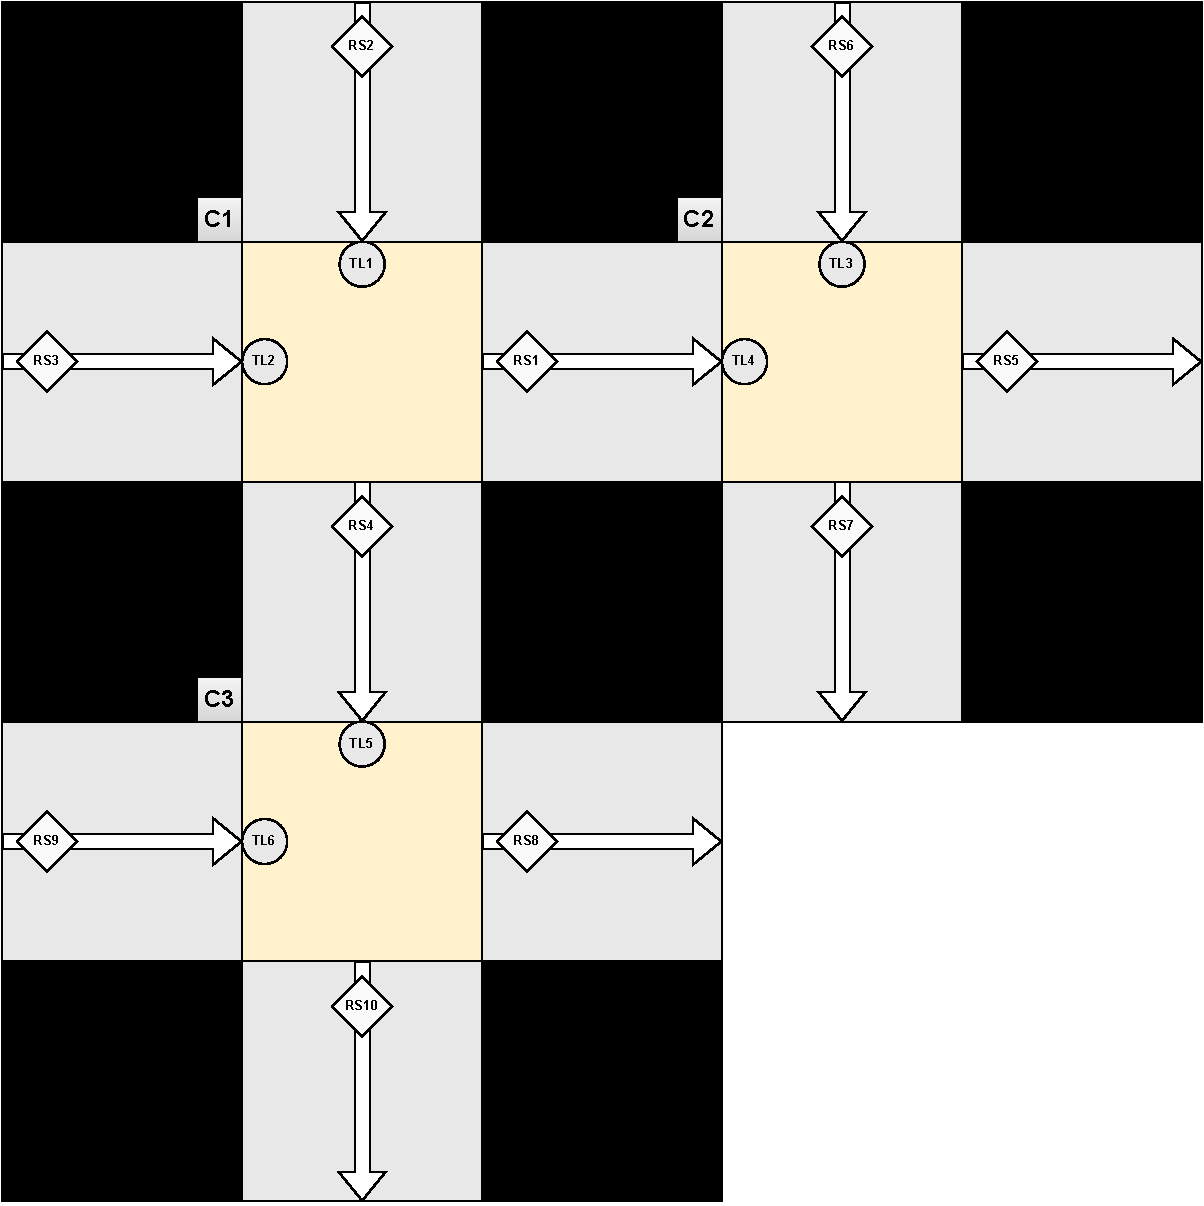
\includegraphics[width=1\linewidth]{text/image/DCruc-CSimple2x1-Topologia.pdf}
    \caption{Topología de la matriz de cruces simples 2x1}
    \label{fig:cruce_simple2x1_topologia}
\end{figure}

\newpage
\section{Ciudad 3. Matriz de cruces simples 2x2}
\begin{figure}[H]
    \centering
    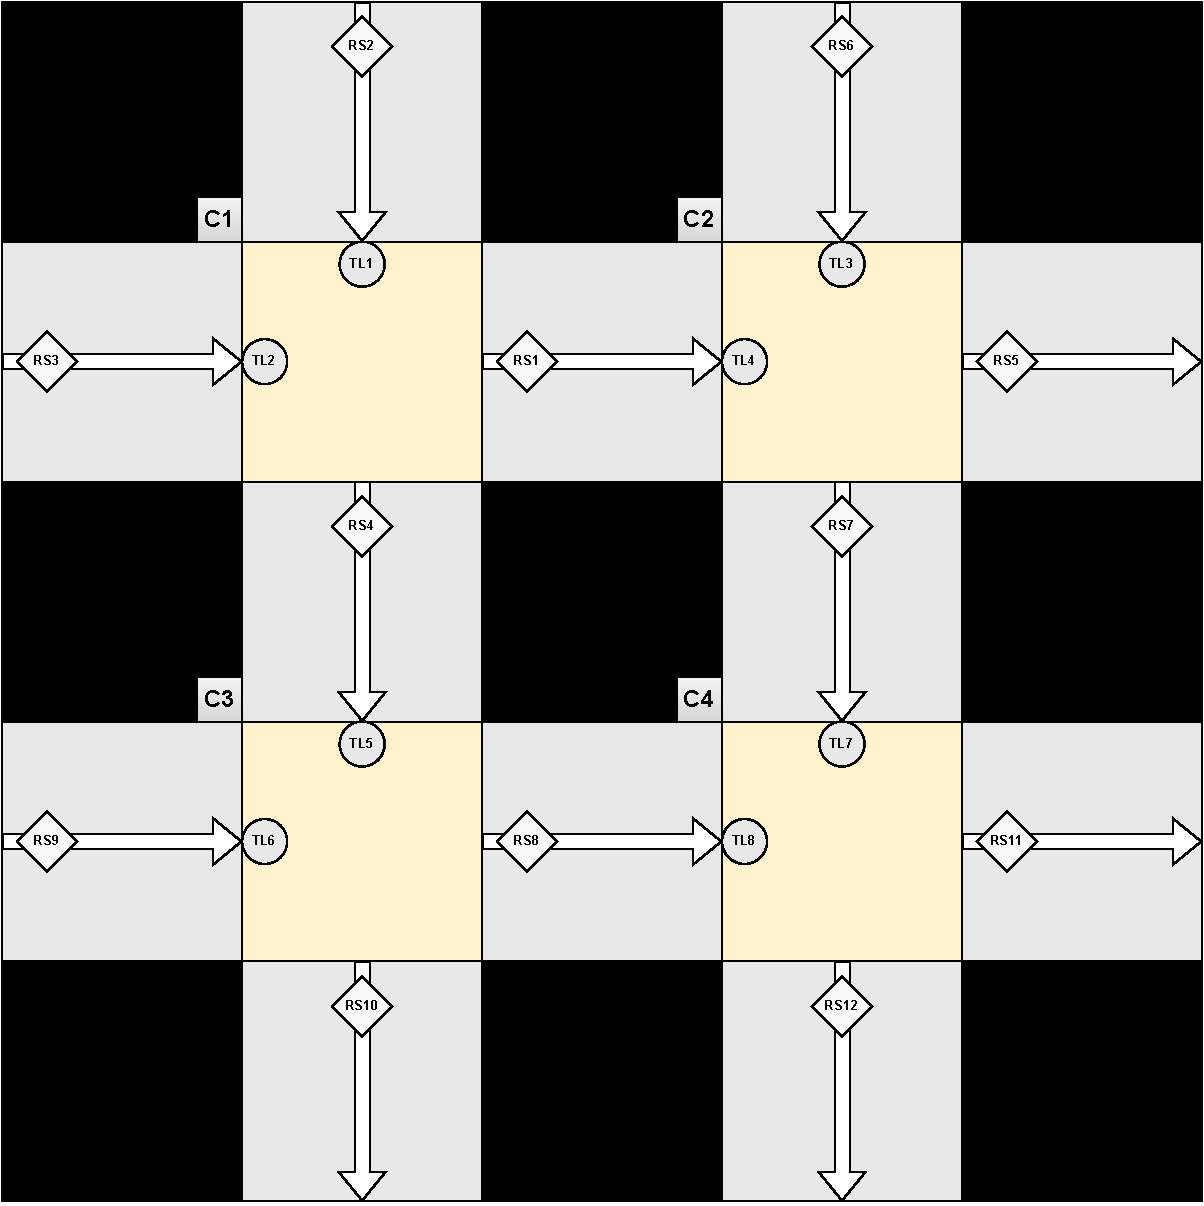
\includegraphics[width=1\linewidth]{text/image/DCruc-CSimple2x2-Topologia.pdf}
    \caption{Topología de la matriz de cruces simples 2x2}
    \label{fig:cruce_simple2x2_topologia}
\end{figure}

\newpage
\section{Ciudad 4. Matriz de cruces simples 3x3}
\begin{figure}[H]
    \centering
    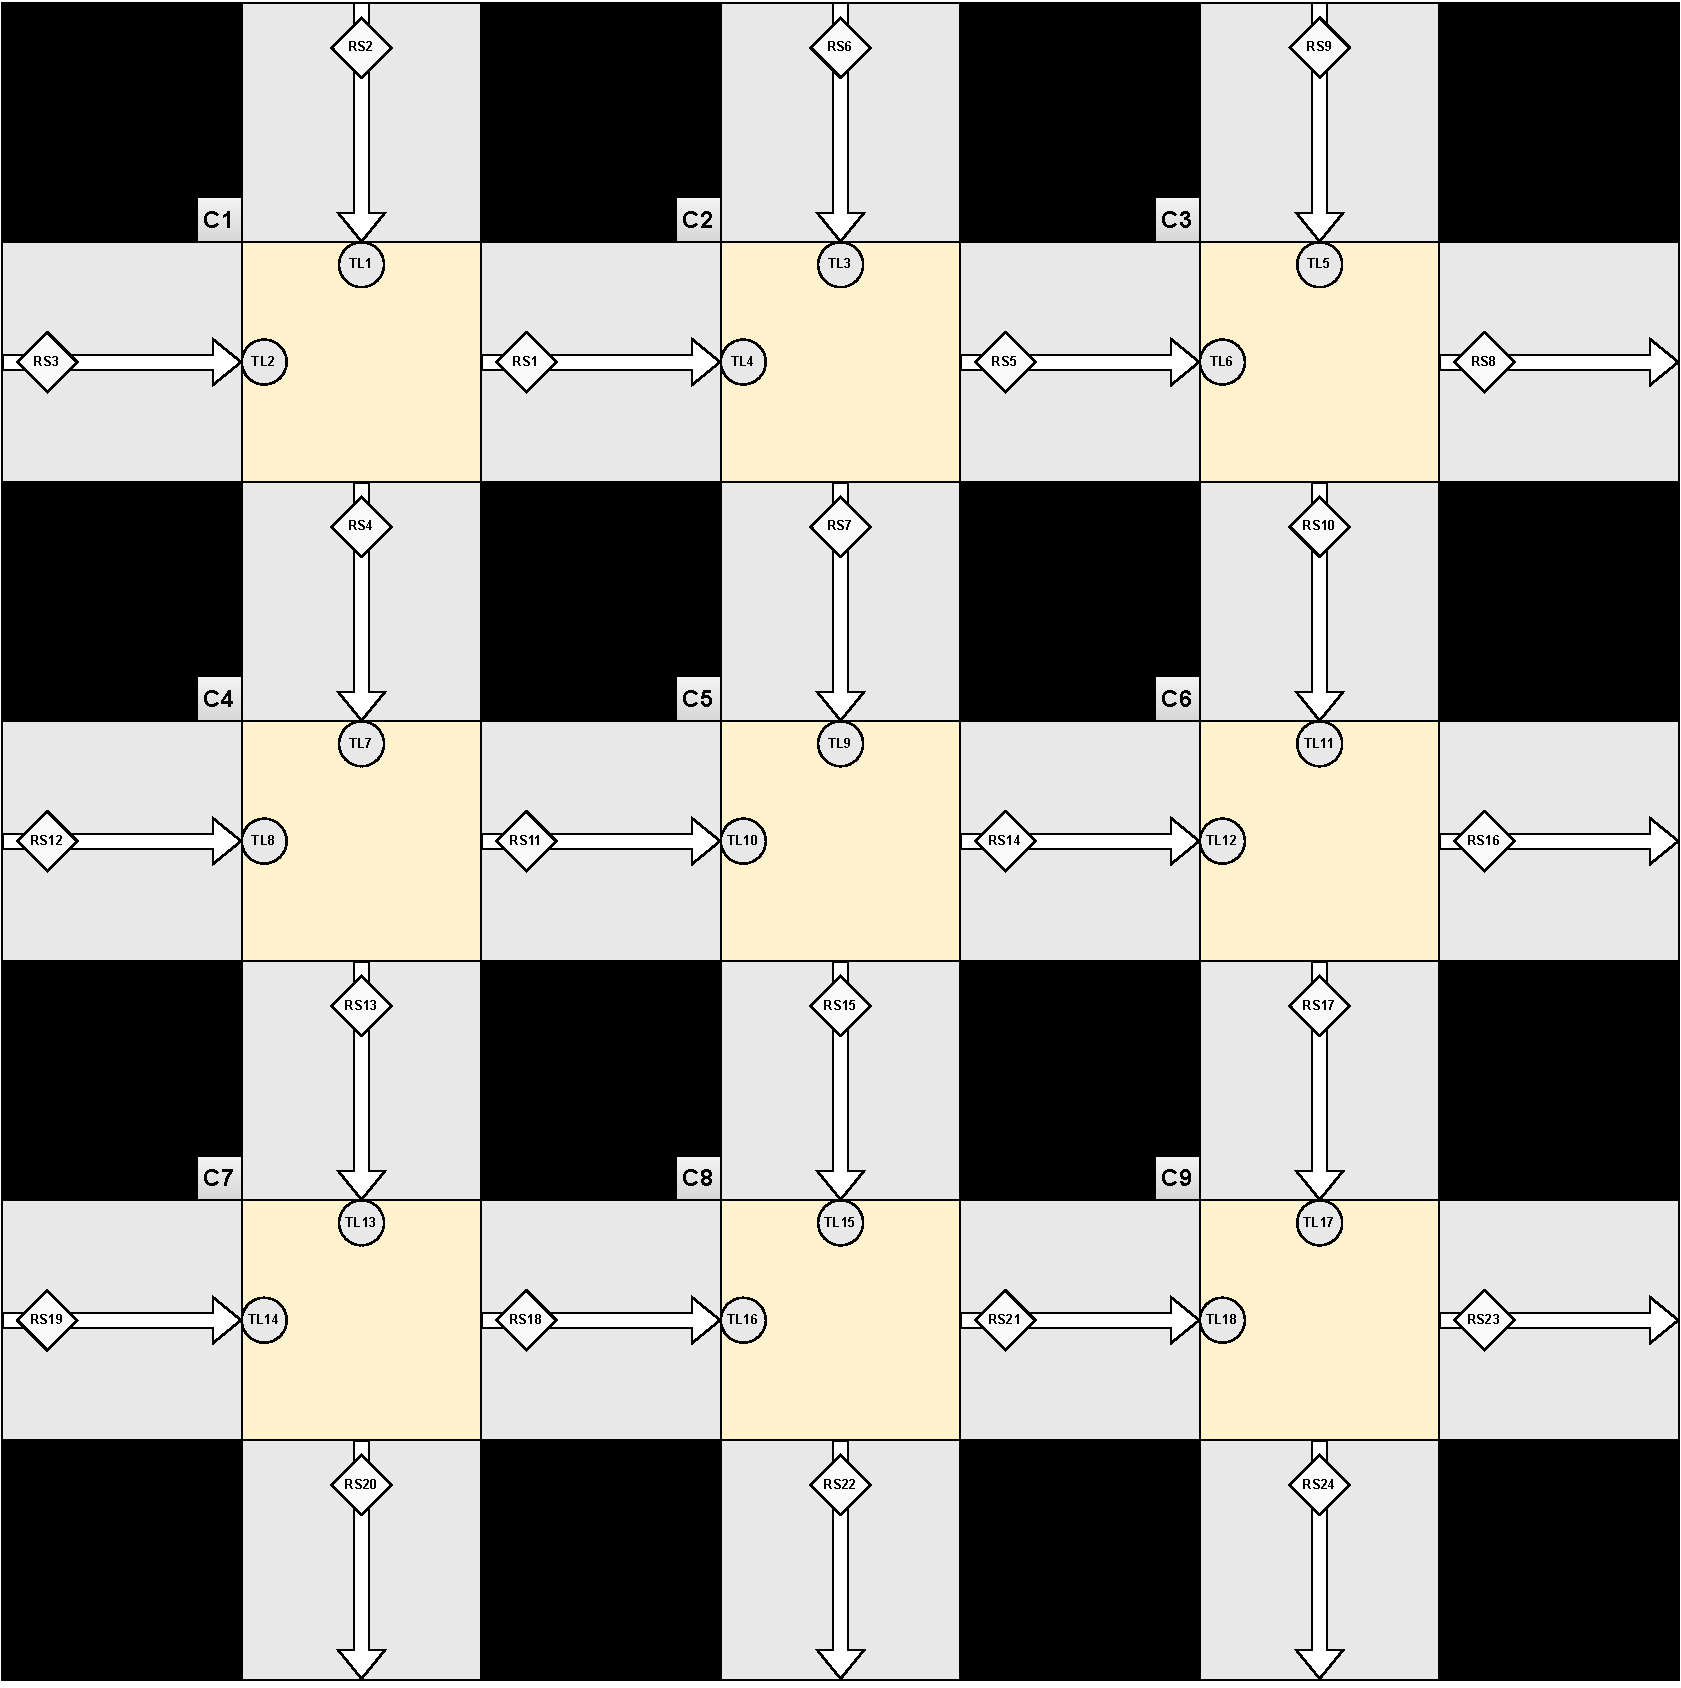
\includegraphics[width=1\linewidth]{text/image/DCruc-CSimple3x3-Topologia.pdf}
    \caption{Topología de la matriz de cruces simples 3x3}
    \label{fig:cruce_simple3x3_topologia}
\end{figure}

\newpage
\section{Ciudad 5. Cruce estándar}
\begin{figure}[H]
    \centering
    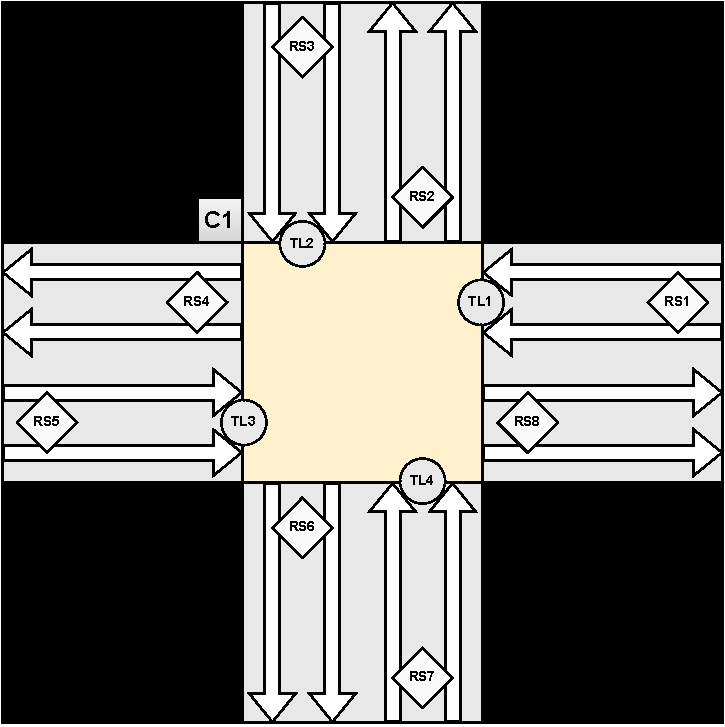
\includegraphics[width=1\linewidth]{text/image/DCruc-CEstandar-Topologia.pdf}
    \caption{Topología del cruce estándar}
    \label{fig:cruce_estandar_topologia}
\end{figure}

\newpage
\section{Ciudad 6. Cruce complejo real}
El cruce de la Avenida de la Constitución con la Avenida Doctor Olóriz y Avenida Andaluces es el escenario real que se ha representado. Es una de las intersecciones más problemáticas y con más tráfico de la ciudad de Granada.
\subsection{Marcación del cruce real}
\begin{figure}[H]
    \centering
    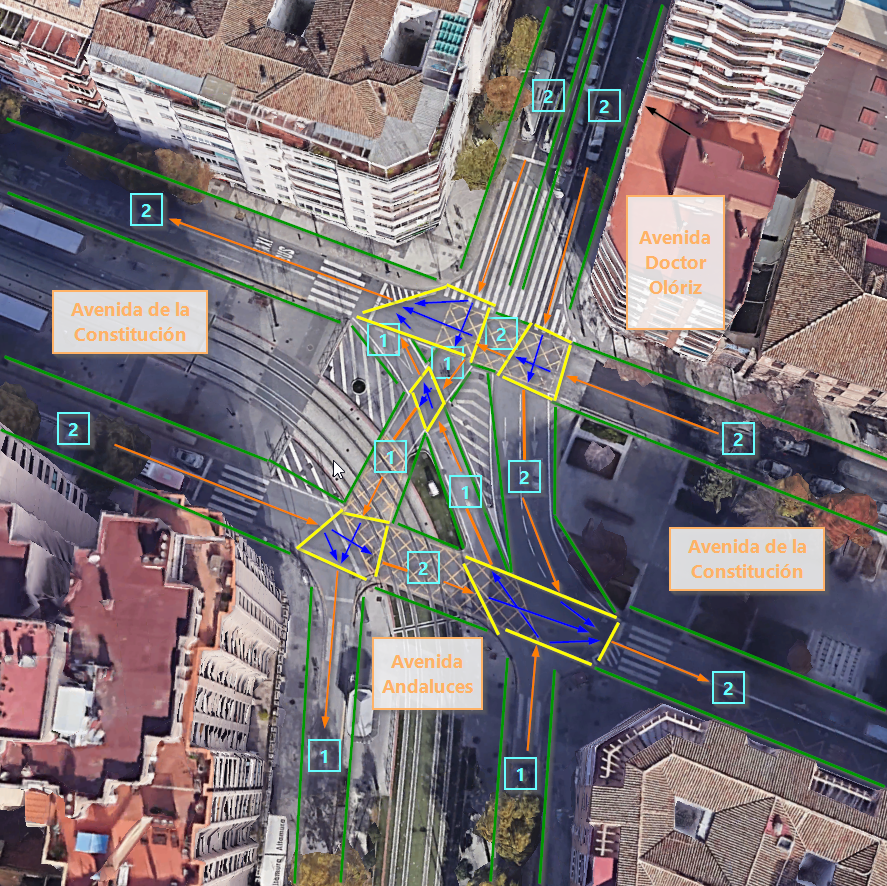
\includegraphics[width=0.95\linewidth]{text/image/DCruc-CReal.png}
    \caption{Cruce real: Avenida de la Constitución, Avenida Doctor Olóriz y Avenida Andaluces}
    \label{fig:cruce_real}
\end{figure}
Como se puede observar, el modelado del escenario consta de cinco cruces (en amarillo), quince tramos de calle (cada par de líneas verdes), doce semáforos (uno por cada tramo de calle de entrada a un cruce) y quince tramos de cruce (en azul).

\newpage
\subsection{Topología del cruce real}
Tras haber pasado el marcado del cruce real a el tipo modelo que se está utilizando, se obtendría la siguiente topología:
\begin{figure}[H]
    \centering
    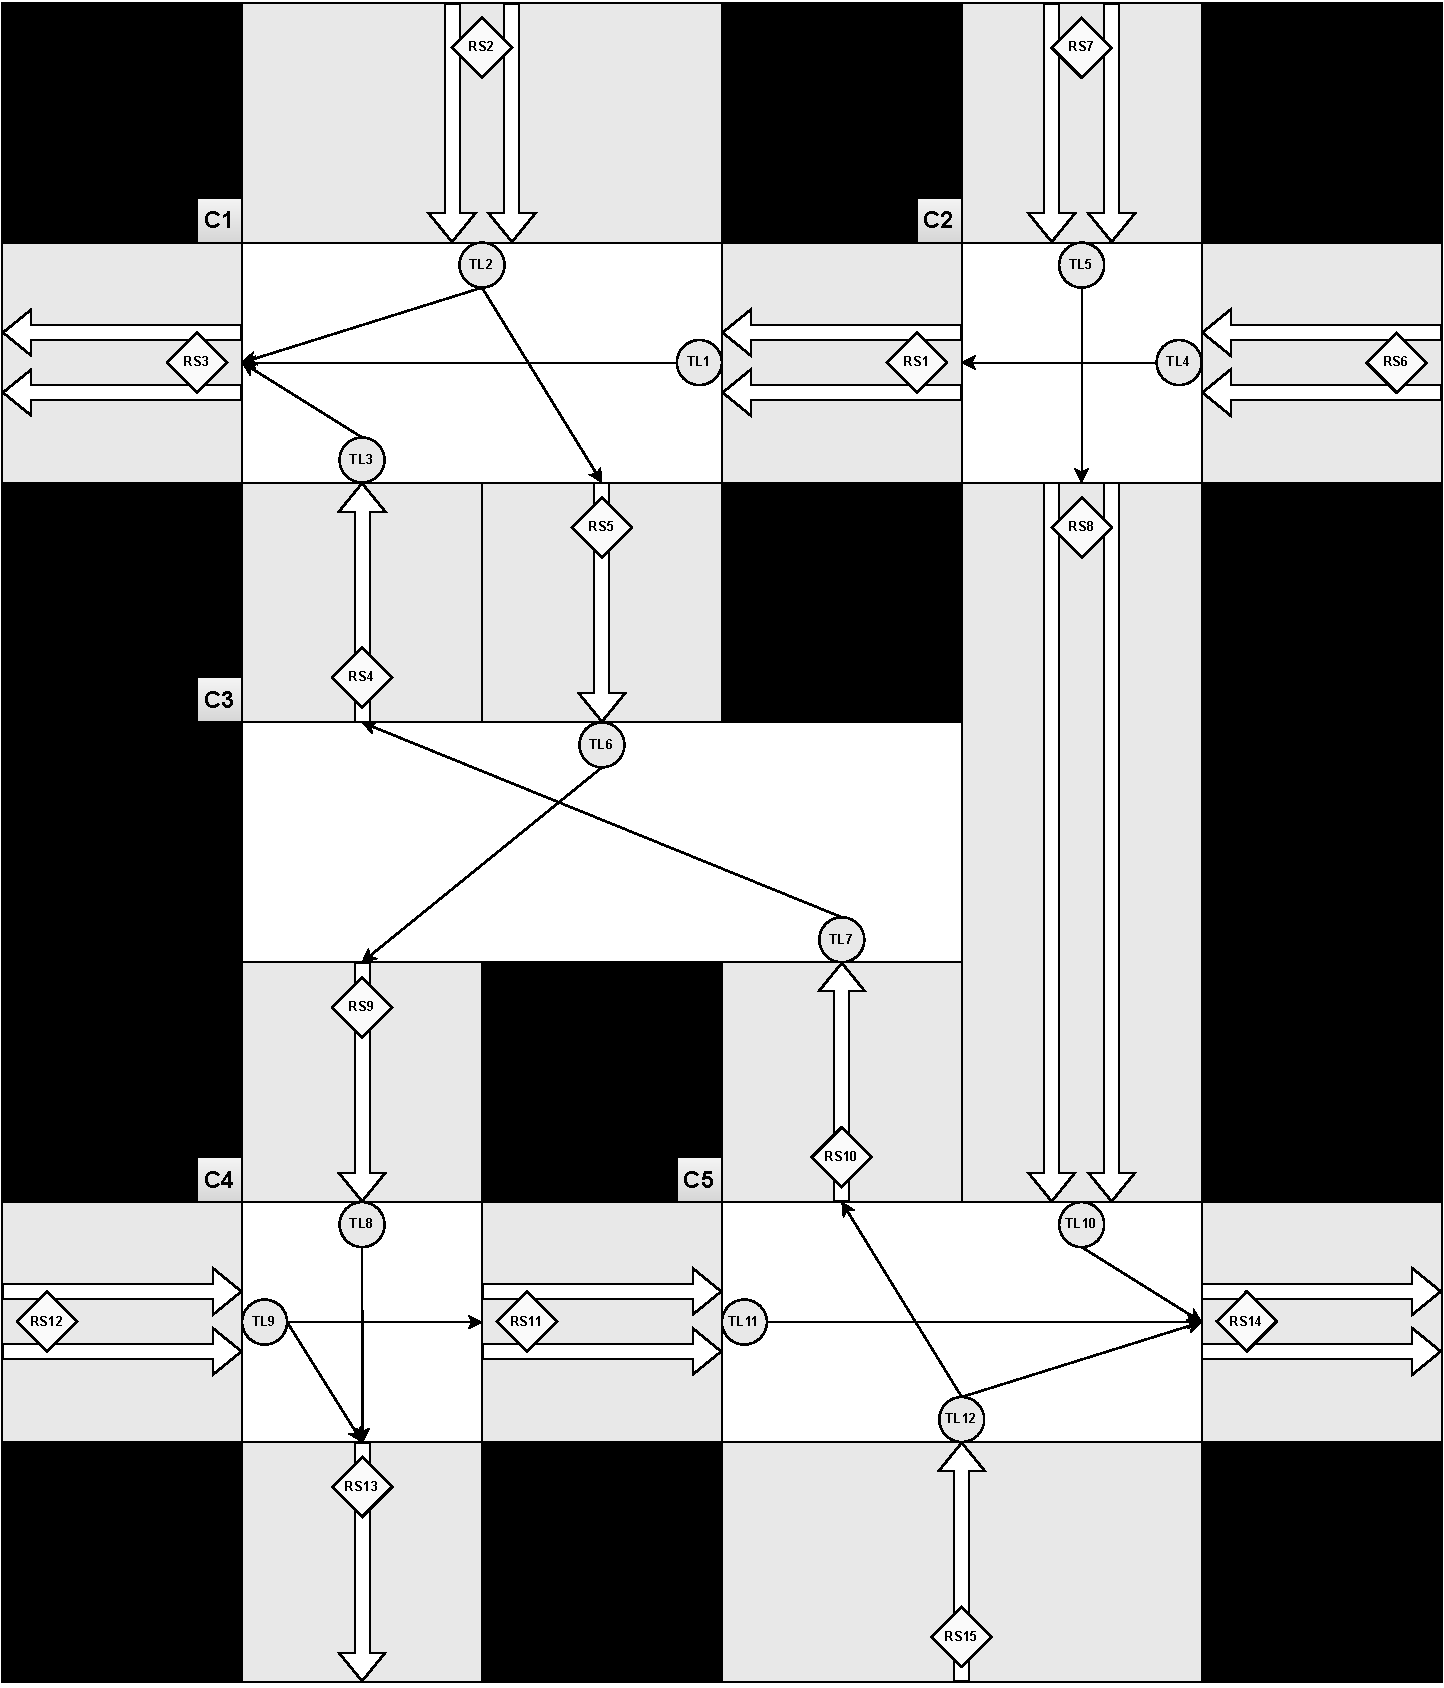
\includegraphics[width=1\linewidth]{text/image/DCruc-CReal-Topologia.pdf}
    \caption{Topología del cruce real: Avenida de la Constitución, Avenida Doctor Olóriz y Avenida Andaluces}
    \label{fig:cruce_real_topologia}
\end{figure}



\chapter{Análisis de los resultados obtenidos}
    \label{chap:seven}
    
\section{Resultados de la simulación de tráfico}
TODO

\newpage
\section{Resultados de seguimiento del proyecto}
Un burndown chart es una gráfica en la que se puede ver el estado del progreso de un proyecto en un sprint, en una release, en el proyecto completo o en aquel período que se haya establecido.

Para construir este gráfico es necesaria determinada información:
\begin{itemize}
    \item \textbf{Tiempo}. Corresponde al eje X de la gráfica. Representa para $x=0$ el inicio del periodo temporal y para $x=t$ el final del periodo temporal. Estos dos valores se corresponden, por ejemplo, en el burndown chart global del proyecto con las fechas de inicio y finalización del mismo.
    \item \textbf{Cantidad de trabajo}. Corresponde al eje Y de la gráfica. Representa el trabajo planificado que se debe realizar durante el tiempo medido. Cuando se estiman las tareas, independientemente de la unidad de estimación que se utilice, se obtiene un valor que indica la cantidad de trabajo a realizar. El valor de cantidad de trabajo restante debe ir decreciendo en relación al tiempo que va avanzando.
    \item \textbf{Referencia ideal}. Corresponde a la línea que diagonal trazada desde la parte superior izquierda hasta la parte inferior derecha. Representa la relación ideal entre la disminución de la cantidad de trabajo y el tiempo que se debería producirse durante el transcurso de la fase correspondiente. Cuanto más se aproxime la línea real a la linea ideal se podría decir que se está trabajando de mejor forma en relación a la consecución de objetivos.
\end{itemize}

Además de lo anterior, si se tiene el conocimiento y la experiencia suficiente trabajando con estas herramientas ágiles, se puede obtener mucha información útil sobre el seguimiento del proyecto. Esta información puede servir, entre otras muchas cosas, para impulsar las buenas prácticas y promover el mismo desarrollo del proyecto. 

\subsection{Burndown chart global del proyecto}
Observando el burndown chart global del proyecto, expuesto en la figura \ref{fig:burndown_chart_proyecto}, se pueden apreciar varias cosas interesantes:
\begin{itemize}
    \item Hay un tramo de la curva totalmente plano. Como posteriormente se explicará, este tramo corresponde a un período en el que no se ha realizado trabajo.
    \item Prácticamente hasta final del proyecto, se ha ido siempre por detrás del trabajo estimado. Sin embargo, esto se debe a algunos periodos en los que se ha trabajado menos, como el mencionado arriba. 
    \item En muchos periodos, como se puede ver, se ha realizado más trabajo del planificado, son los períodos en los que la línea roja se aproxima más a la línea azul.
    \item Desde la mitad del proyecto en adelante, aproximadamente, se ha realizado más trabajo del planificado. Esto ha conseguido compensar la diferencia que se había producido anteriormente.
\end{itemize}
Se puede concluir con que, de forma global, se ha realizado la cantidad de trabajo planificada antes de lo previsto. Además, pese a la diferencia existente en algunos puntos con para la situación ideal, se ha logrado mantener bajo control el proyecto durante los diferentes sprints. Gracias a este seguimiento se han podido valorar en cada momento los riesgos existentes y se han tomando acciones en relación a estos, por ejemplo, en forma de compensación de trabajo siempre que ha sido necesario debido a las horas no realizadas en periodos anteriores.

\begin{figure}[H]
    \centering
    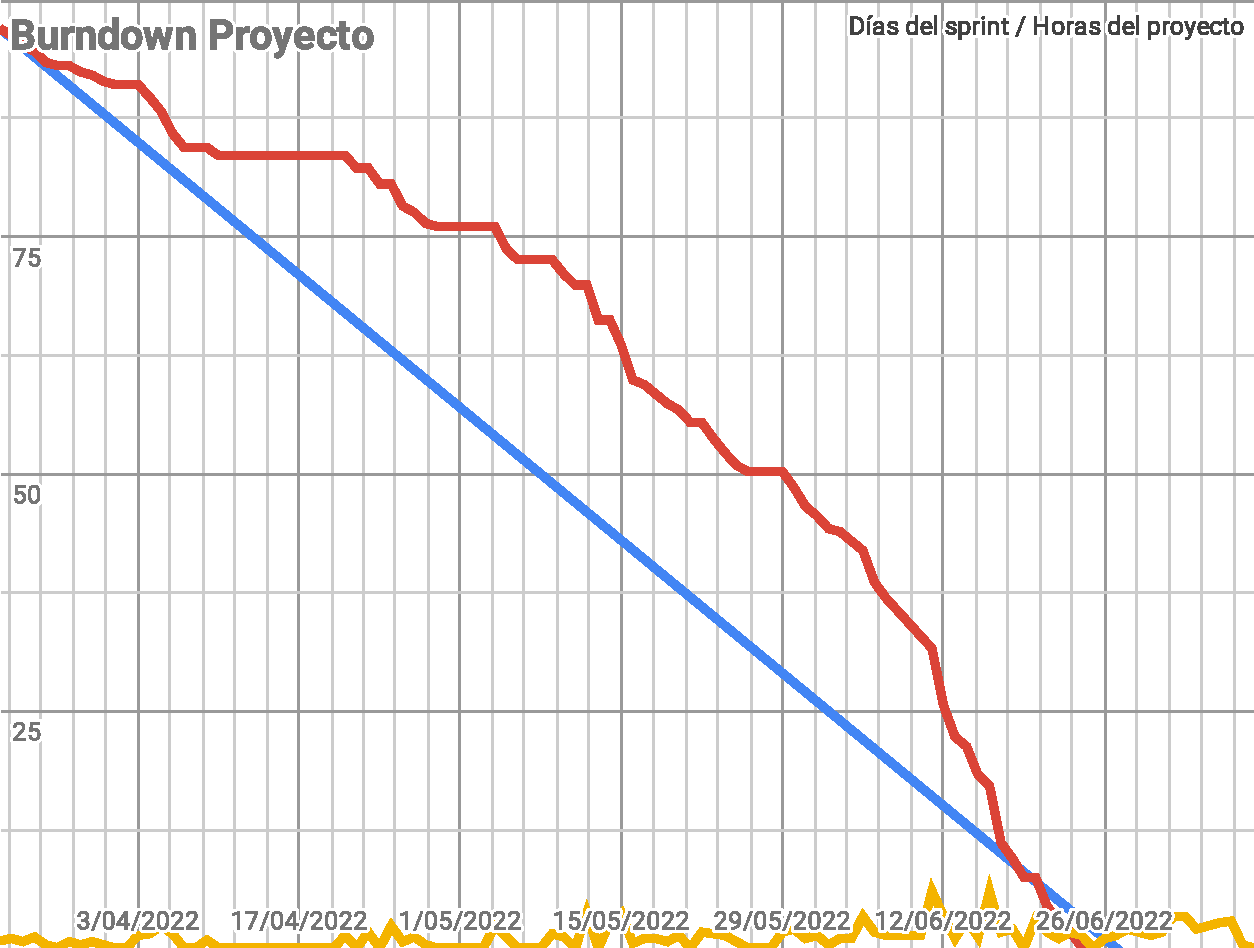
\includegraphics[width=1\linewidth]{text/image/BurndownChartGlobal.pdf}
    \caption{Burndown chart $|$ Proyecto $|$ del 22/03 al 08/07}
    \label{fig:burndown_chart_proyecto}
\end{figure}

\newpage
\subsection{Burndown charts de cada sprint}
Durante el transcurso de cada sprint, se ha realizado el seguimiento tanto particular de dicho sprint como global de todo el proyecto. Gracias a esto, se ha podido tener una perspectiva global de la evolución del mismo.

\paragraph{Sprint 1 (del 22/03 al 05/04)} 
Durante los primeros días del sprint se mantuvo un trabajo constante en relación a lo que estaba previsto. Tras esto, la cantidad de trabajo realizada se redujo y, aun trabajando diariamente, la cantidad de trabajo realizada no era suficiente. Al final del sprint aumentó de nuevo el trabajo diario realizado, sin embargo, no se pudo completar toda la cantidad de trabajo prevista para el sprint.
\begin{figure}[H]
    \centering
    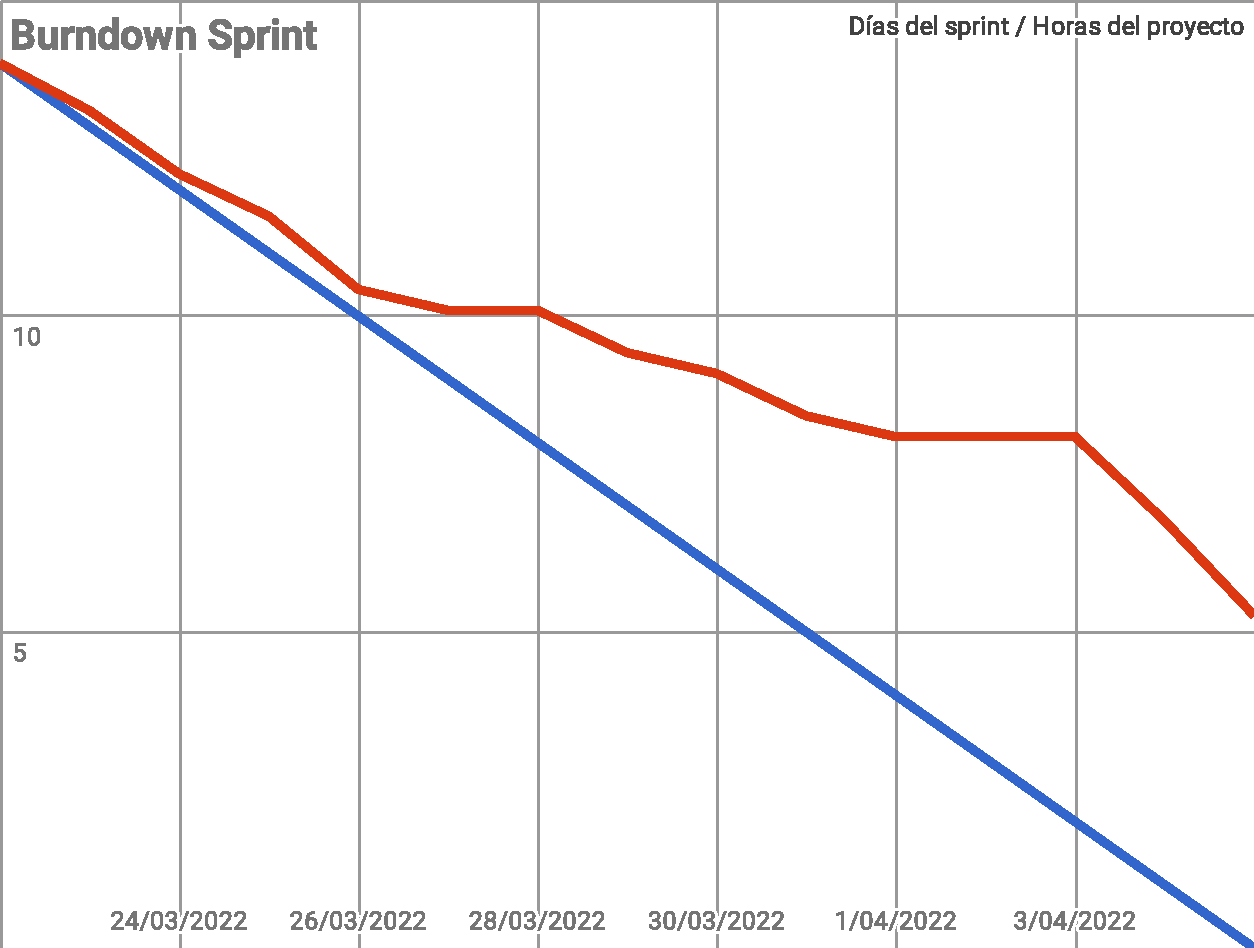
\includegraphics[width=1\linewidth]{text/image/BurndownChart1.pdf}
    \caption{Burndown chart $|$ Sprint 1 $|$ del 22/03 al 05/04}
    \label{fig:burndown_chart_1}
\end{figure}

\newpage
\paragraph{Sprint 2 (del 06/04 al 20/04)}
Este sprint es algo totalmente anormal, que no se debe dar. La razón es simple, si la línea roja permanece horizontal es porque no se está trabajando. No obstante, es correcto porque inicialmente se planificó que durante el periodo vacacional de Semana Santa no se iba a trabajar. Habría sido interesante omitir este periodo del seguimiento, sin embargo, se ha considerado interesante para mostrar una tendencia mala en relación al desarrollo del proyecto.
\begin{figure}[H]
    \centering
    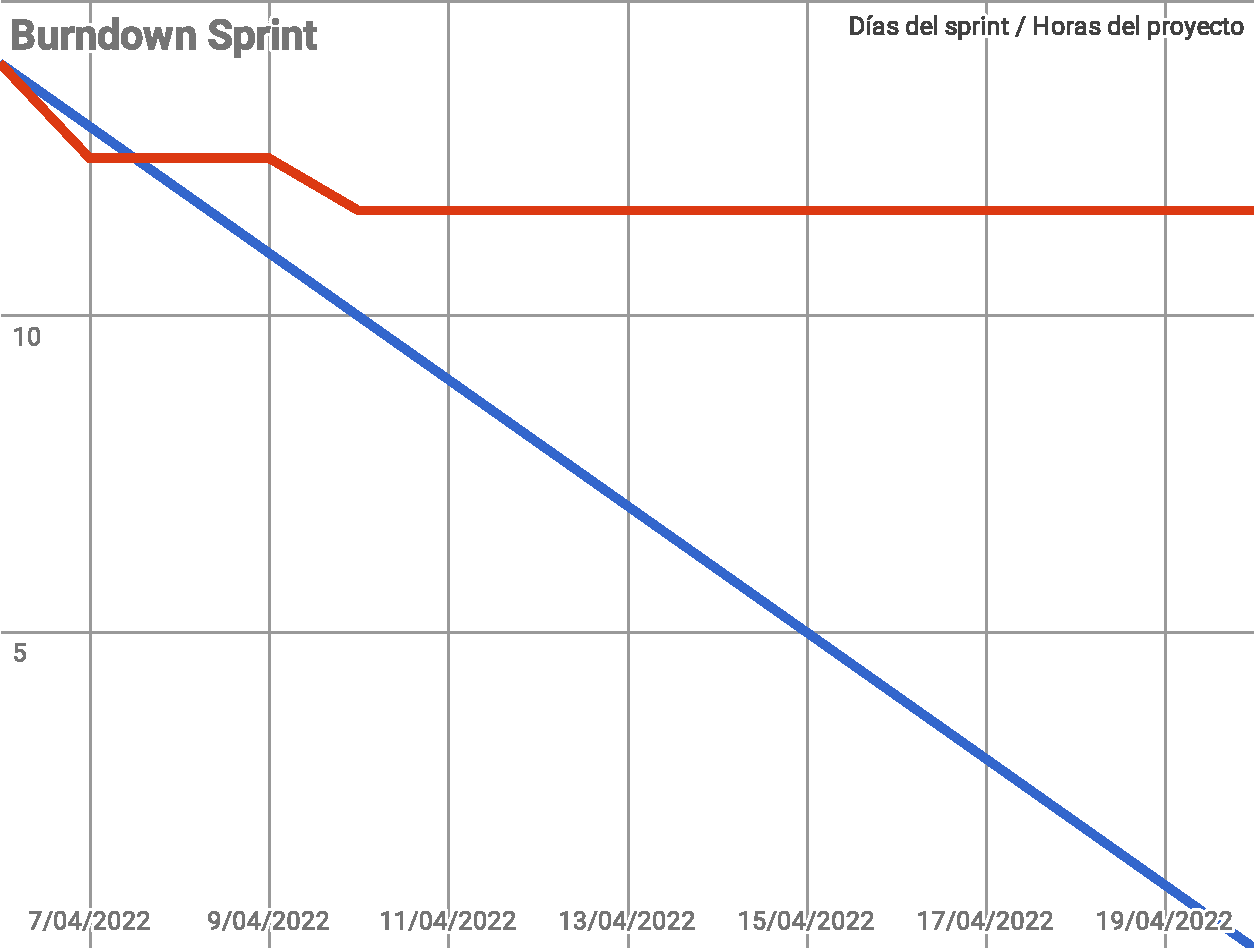
\includegraphics[width=1\linewidth]{text/image/BurndownChart2.pdf}
    \caption{Burndown chart $|$ Sprint 2 $|$ del 06/04 al 20/04}
    \label{fig:burndown_chart_2}
\end{figure}

\newpage
\paragraph{Sprint 3 (del 21/04 al 05/05)}
Se puede apreciar que la tendencia es muy buena durante la primera parte del sprint. Hasta la mitad del periodo la curva roja se sitúa alrededor de la tendencia ideal, lo cual manifiesta que el sprint está controlado. Posteriormente, se puede observar un parón hasta el día previo a la finalización del sprint, donde se realizó una cantidad de trabajo considerable.
\begin{figure}[H]
    \centering
    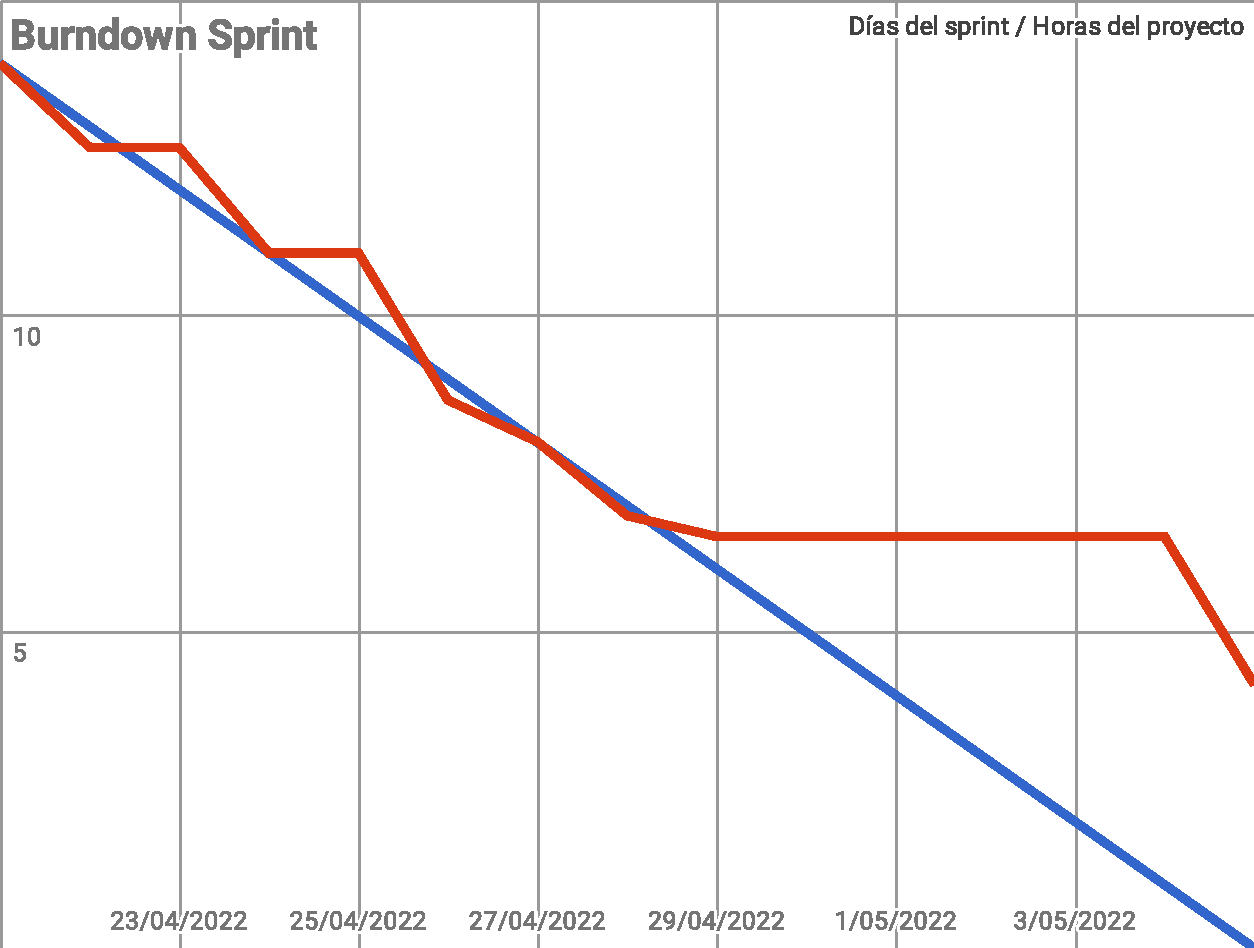
\includegraphics[width=1\linewidth]{text/image/BurndownChart3.pdf}
    \caption{Burndown chart $|$ Sprint 3 $|$ del 21/04 al 05/05}
    \label{fig:burndown_chart_3}
\end{figure}

\newpage
\paragraph{Sprint 4 (del 06/05 al 20/05)}
El gráfico de este sprint muestra que se realizaron grandes cantidades de trabajo en días concretos. Se puede apreciar que algo después de pasar la mitad del tiempo del sprint, se consiguió cortar la curva ideal con la curva de trabajo real, realizando en los días anteriores y posteriores mucha más cantidad de trabajo de la que estaba planificada. Esto, en cierto modo, sirvió para compensar parte del trabajo no realizado en sprints anteriores.
\begin{figure}[H]
    \centering
    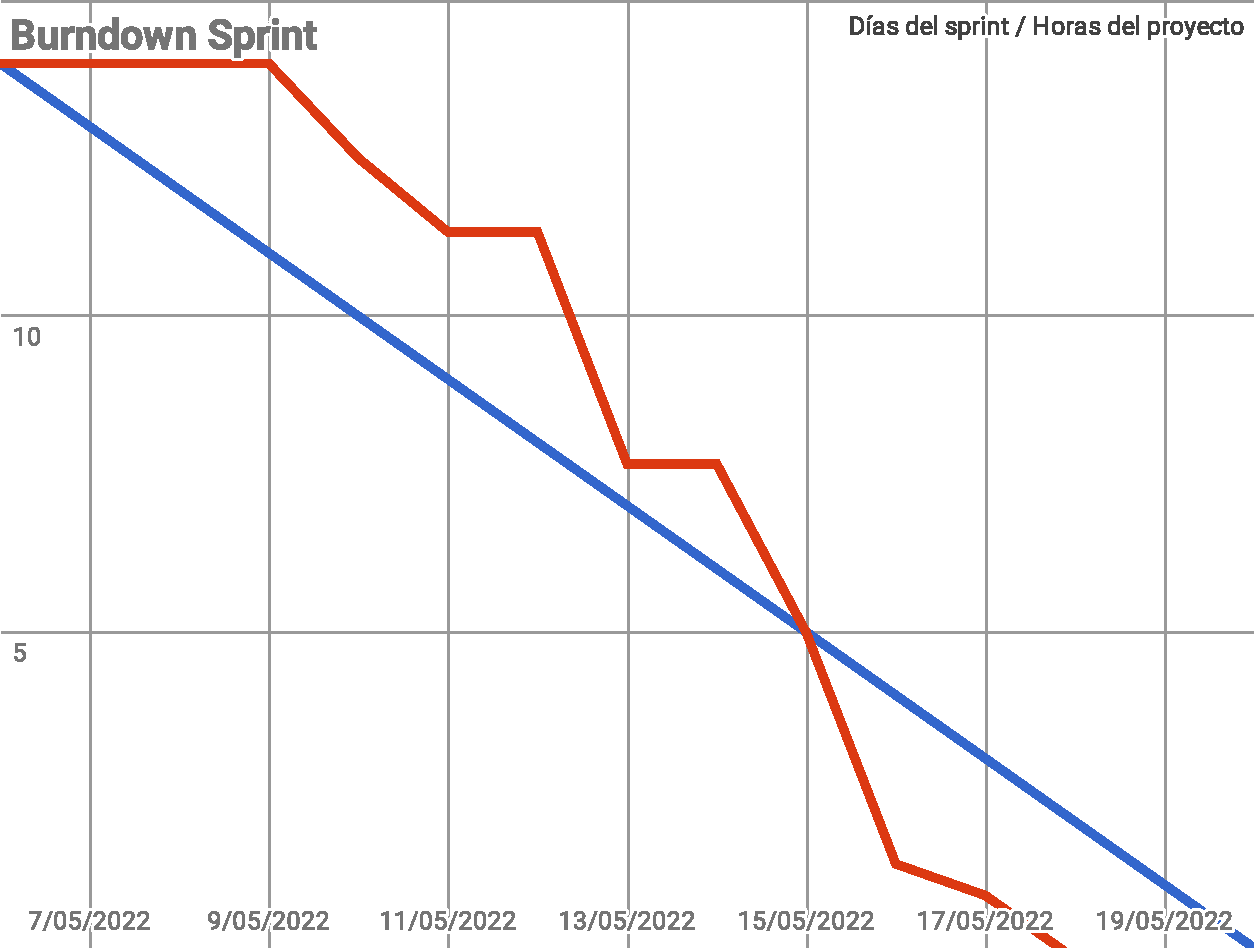
\includegraphics[width=1\linewidth]{text/image/BurndownChart4.pdf}
    \caption{Burndown chart $|$ Sprint 4 $|$ del 06/05 al 20/05}
    \label{fig:burndown_chart_4}
\end{figure}

\newpage
\paragraph{Sprint 5 (del 21/05 al 04/06)}
Durante el presente sprint, se mantuvo una tendencia adecuada hasta, aproximadamente, un poco antes de la mitad del mismo. A partir de ese momento hubo un par de días de parón, los cuales, posteriormente, se compensaron en casi su totalidad.
\begin{figure}[H]
    \centering
    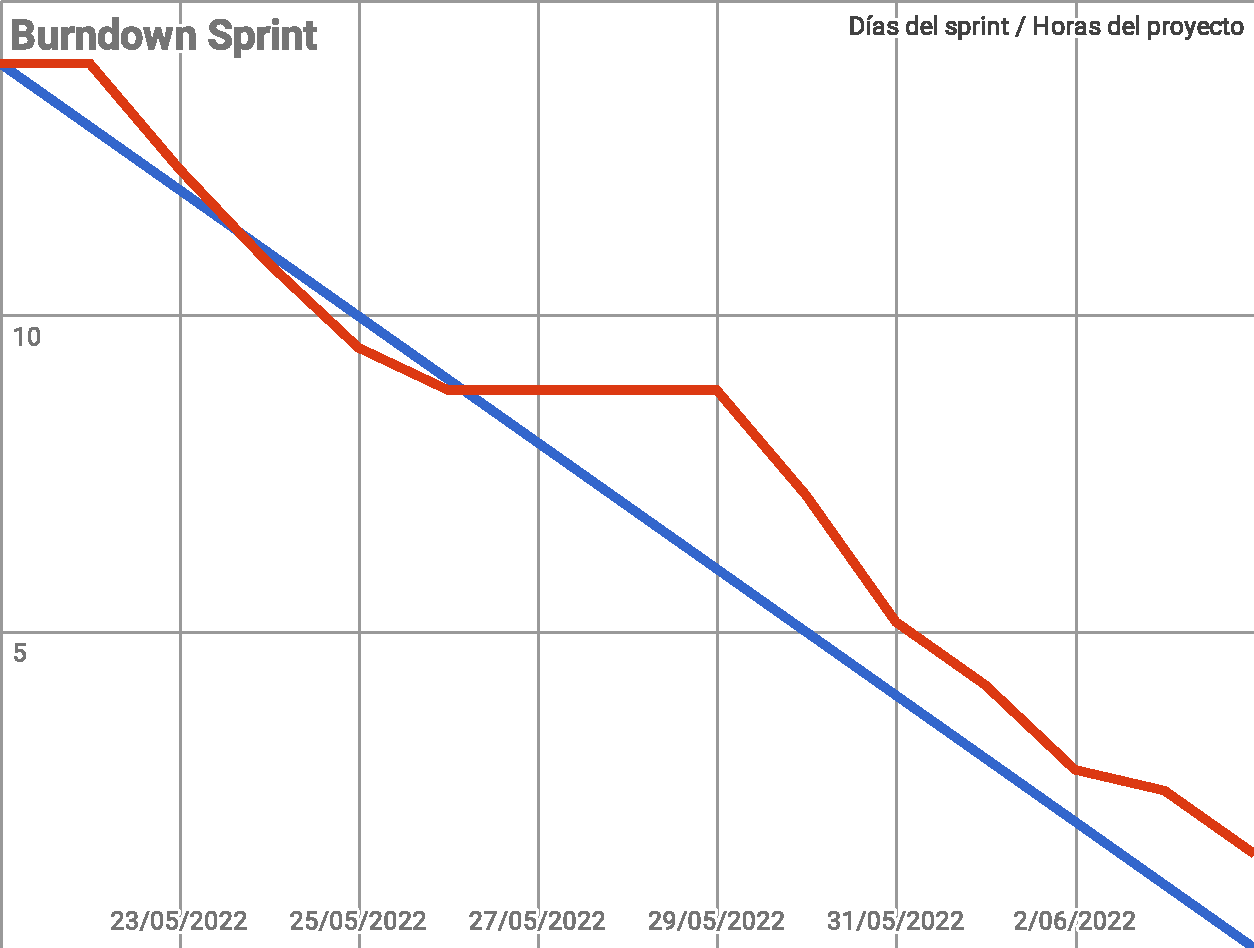
\includegraphics[width=1\linewidth]{text/image/BurndownChart5.pdf}
    \caption{Burndown chart $|$ Sprint 5 $|$ del 21/05 al 04/06}
    \label{fig:burndown_chart_5}
\end{figure}

\newpage
\paragraph{Sprint 6 (del 05/06 al 19/06)}
Claramente, se puede ver que en este sprint se realizó una cantidad de trabajo mucho más alta de lo que estaba planificado. Sin embargo, si se analiza desde un punto de vista global, se puede entender que al acercarse el final de proyecto es necesario invertir más tiempo y compensar la cantidad de trabajo que en sprints anteriores no se llegó a completar.
\begin{figure}[H]
    \centering
    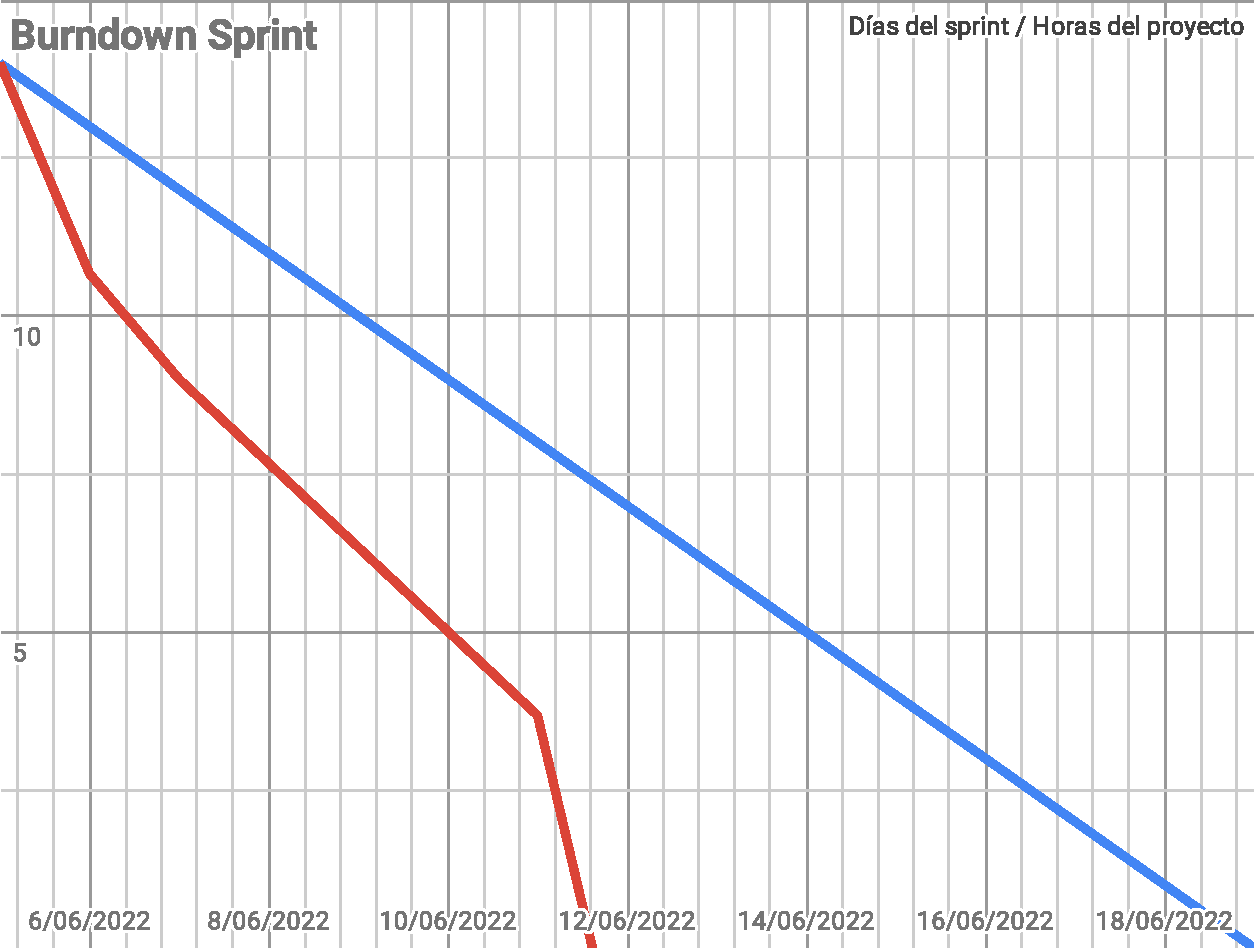
\includegraphics[width=1\linewidth]{text/image/BurndownChart6.pdf}
    \caption{Burndown chart $|$ Sprint 6 $|$ del 05/06 al 19/06}
    \label{fig:burndown_chart_6}
\end{figure}

\newpage
\paragraph{Sprint 7 (del 20/06 al 04/07)}
De manera similar al sprint anterior, se puede ver que en este sprint se realizó una cantidad de trabajo mucho más alta de lo que estaba planificado. Si que comparan ambos diagramas se puede apreciar que la tendencia es muy parecida. Esto se debe a que al ser parte de la fase final del proyecto se realizaron todas las horas de trabajo necesarias para finalizarlo.
\begin{figure}[H]
    \centering
    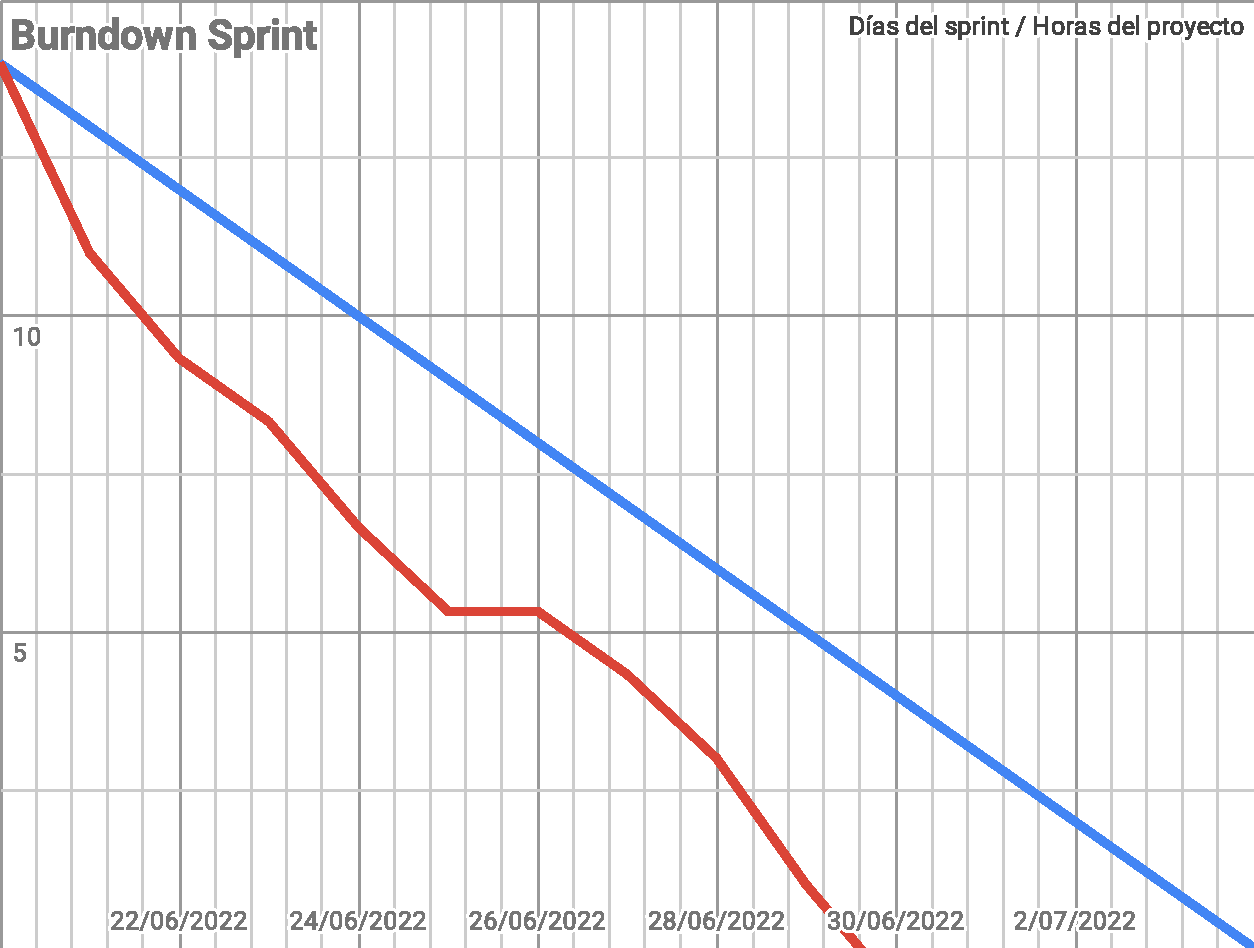
\includegraphics[width=1\linewidth]{text/image/BurndownChart7.pdf}
    \caption{Burndown chart $|$ Sprint 7 $|$ del 20/06 al 04/07}
    \label{fig:burndown_chart_7}
\end{figure}

\newpage
\paragraph{Sprint 8 (del 05/07 al 08/07)}
Este sprint posee una duración menor a las dos semanas habituales de sprints anteriores. Esto es debido a que es el último sprint del proyecto, el conocido como sprint de finalización. En este sprint el trabajo realizado va en relación a los últimos preparativos, correcciones y mejoras necesarios para cerrar y entregar el proyecto.
\begin{figure}[H]
    \centering
    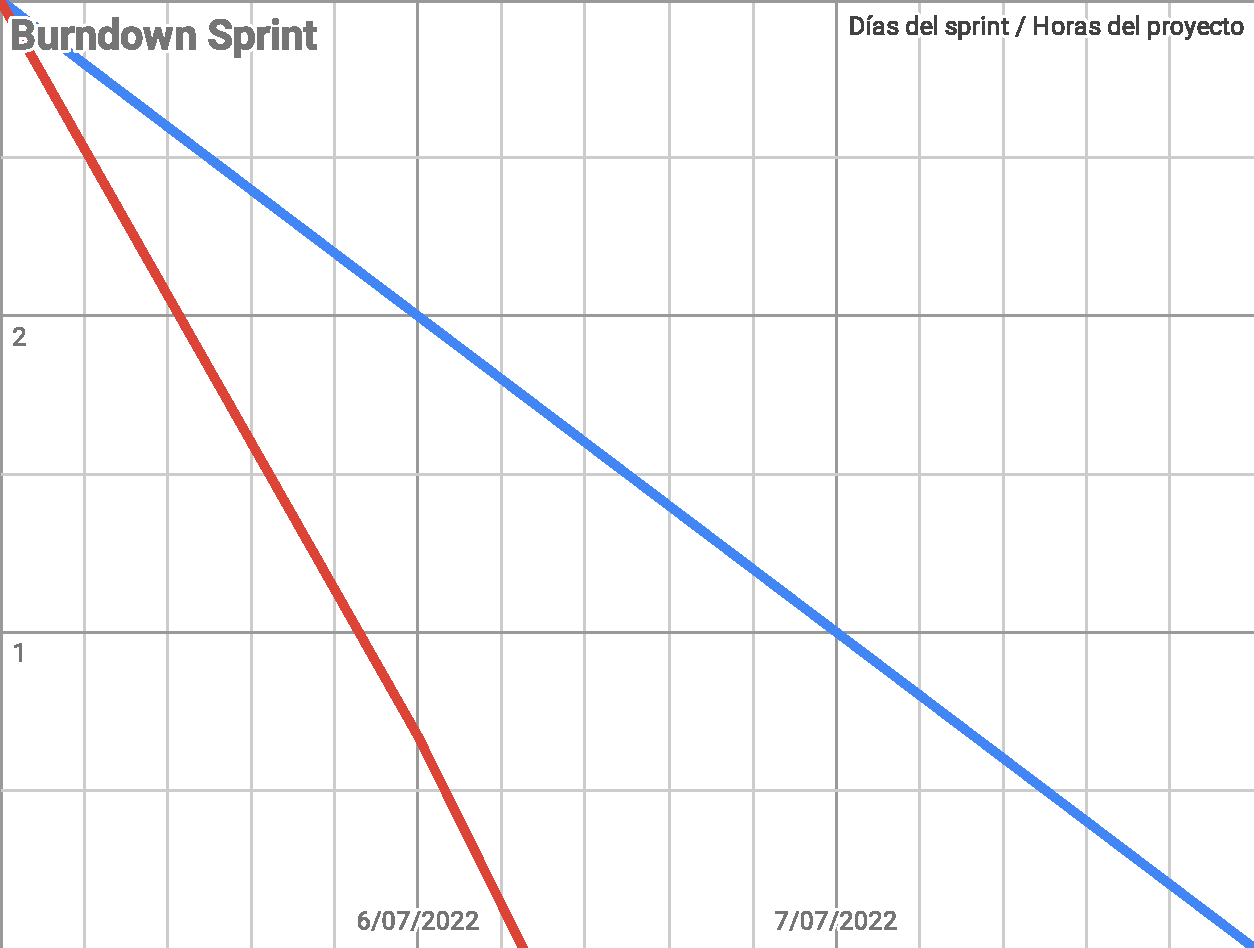
\includegraphics[width=1\linewidth]{text/image/BurndownChart8.pdf}
    \caption{Burndown chart $|$ Sprint 8 $|$ del 05/07 al 08/07}
    \label{fig:burndown_chart_8}
\end{figure}